\section{Experiments}
\label{sec:exp}

\subsection{Data Collection}
\label{sec:datacollection}

We are using ROpenDota by Rosdyana Kusuma to built our data set. ROpenDota is an API wrapper service for OpenDota in R. We labeling players from replay and the replay based on The International 2016 and Kiev Major, which contains 8419 labeled players. Using replay data from professional players will guarantee our data set from low level data.

\subsection{Attribute Construction and Evaluation}
\label{sec:attconsandeval}
Attributes for evaluation is presented in table 1. While some attributes correspond directly to summary data, attributes that capture positional information the fighting behavior require more complex processing of the replay data. Different attribute filters implemented in the Java library WEKA \cite{hall2009weka} to determine the best set of attributes. Our results with the \textit{WtrapperSubsetEval} class with best-first search are presented in table 1. We have chosen this algorithm for our final attribute selection because it resulted in the highest accuracy with our labeled data set. For classification we selected all attributes that were present in at least four folds, excluding assists, as this resulted in the overall highest accuracy. In the following sections we describe the algorithms and heuristics we developed to calculate the attributes that cannot be directly obtained from replay files. They can be grouped into five rough categories: space and movement, early ganks, team fights, support items, and damage types. Not all of the attributes we describe in this section were finally chosen to be used for classification within this work but they might prove valuable for future works.

\subsection{Space and Movement}
\label{spaceandmovement}
% figures
\begin{figure}
\centering
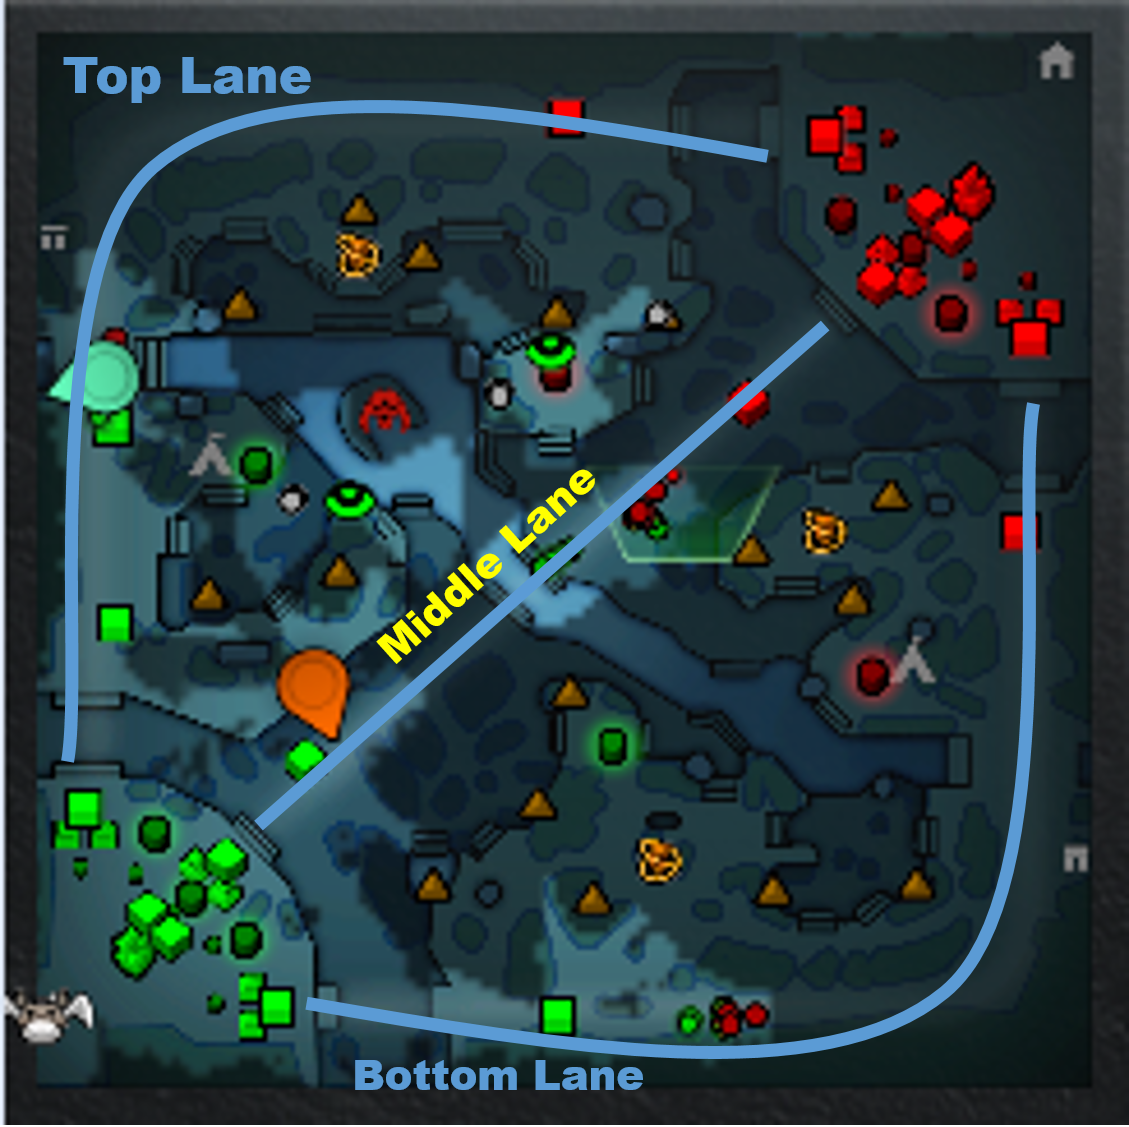
\includegraphics[width=2.5in]{./figures/lane_map.png}
\caption{\textit{Dota 2} map designed with three lane. Top lane, middle lane and also bottom lane.}
\label{fig:map_lane}
\end{figure}

Most of player roles depend on the lane (see figure \ref{fig:map_lane}) which is the most active in the early game. Player lane information also provides the constructor for the other attributes, e.g., the \textit{lane partners}. 
